\documentclass[dvisvgm,tikz]{standalone}

\usepackage[sfdefault]{inter}
\usetikzlibrary{shapes.geometric, arrows.meta, positioning, calc, fit, decorations.pathmorphing}

%%%%%%%%%%%%%%%%%%%%%%%%%%%%%%%%%%%%%%%%%%%%%%%%%%%
%Colors
% Warm gray to turquoise
\definecolor{warm_gray}{RGB}{128, 120, 115}
\definecolor{sage_gray}{RGB}{110, 125, 120}
\definecolor{pewter}{RGB}{91, 112, 114}
\definecolor{slate_blue}{RGB}{72, 107, 115}
\definecolor{steel_teal}{RGB}{53, 118, 125}
\definecolor{teal}{RGB}{27, 136, 140}
\definecolor{deep_aqua}{RGB}{15, 152, 155}
\definecolor{peacock_blue}{RGB}{0, 167, 171}
\definecolor{blue_green}{RGB}{0, 181, 185}
\definecolor{turquoise}{RGB}{0, 195, 200}

\definecolor{mygray}{gray}{0.9}

% Match our established color scheme
\definecolor{atoken}{RGB}{255, 152, 0}        % Orange for A token
\definecolor{gtoken}{RGB}{76, 175, 80}        % Green for G token
\definecolor{mainblue}{RGB}{74, 144, 226}     % Blue for A classes
\definecolor{maingreen}{RGB}{102, 187, 106}   % Light green for G classes
\definecolor{timegray}{RGB}{158, 158, 158}    % Gray for time component
%%%%%%%%%%%%%%%%%%%%%%%%%%%%%%%%%%%%%%%%%%%%%%%%%%%

\def \G {\textbf{G}}
\def \A {\textbf{A}}
\def \Q {\textbf{Q}}
\def \C {\textbf{C}}
\def \CC {\textbf{C*}}
\def \KA {\textbf{KLIMA}}
\def \KG {\textbf{KlimaX}}

\def \AG {$\overline{\textbf{AG}}$}
\def \AQ {$\overline{\textbf{AQ}}$}

\begin{document}
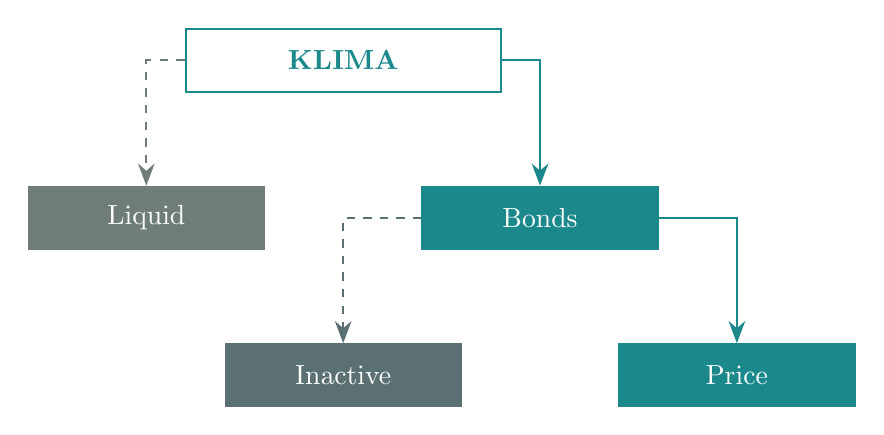
\begin{tikzpicture}[
    staking/.style={
        rectangle,
        draw=teal,
        thick,
        minimum width=4cm,
        minimum height=0.8cm,
        text=teal,
        align=center
    },
    dimension/.style={
        rectangle,
        draw=#1,
        fill=#1,
        text=white,
        minimum width=3cm,
        minimum height=0.8cm,
        align=center
    },
    arrow/.style={
        -{Stealth[length=8pt]},
        thick, #1,
    }
]

% Main staking node
\node[staking] (staking) at (0,2) {\KA{}};

% Dimension nodes
\node[dimension=sage_gray] (unstaked) at (-2.5,0) {Liquid};
\node[dimension=teal] (time) at (2.5,0) {Bonds};

\node[dimension=teal] (price) at (5,-2) {Price};
\node[dimension=pewter] (passive) at (0,-2) {Inactive};

% Draw connecting arrows
\draw[arrow=sage_gray,dashed] (staking.west) -| (unstaked.north);
\draw[arrow=teal] (staking.east) -| (time.north);

\draw[arrow=pewter,dashed] (time.west) -| (passive.north);
\draw[arrow=teal] (time.east) -| (price.north);

\end{tikzpicture}
\end{document}
